\documentclass[tikz,border=8pt]{standalone}
\usepackage{xcolor}
\usetikzlibrary{calc,arrows.meta,backgrounds}
\definecolor{bg}{HTML}{1B1F27}
\definecolor{fg}{HTML}{E6EDF3}
\definecolor{dim}{HTML}{9AA5B1}
\definecolor{c1}{HTML}{7BC47F}
\definecolor{c2}{HTML}{E5826F}
\definecolor{hid}{HTML}{6EA8FE}
\definecolor{ya}{HTML}{F0C060}
\definecolor{yb}{HTML}{B39DDB}
\begin{document}
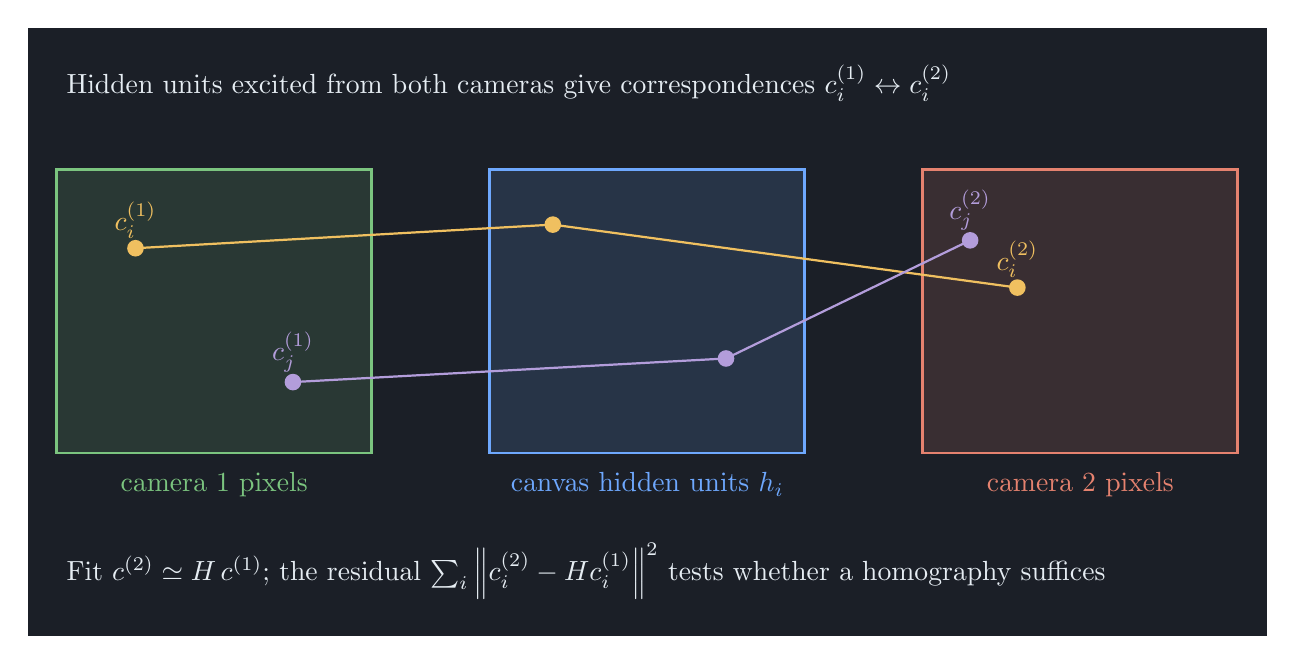
\begin{tikzpicture}[show background rectangle, background rectangle/.style={fill=bg}, inner frame sep=10pt, every node/.style={text=fg}]
\draw[c1, line width=1pt, fill=c1!15!bg] (0,0) rectangle (4,3.6);
\node[text=c1] at (2,-0.4) {camera 1 pixels};
\draw[hid, line width=1pt, fill=hid!15!bg] (5.5,0) rectangle (9.5,3.6);
\node[text=hid] at (7.5,-0.4) {canvas hidden units $h_i$};
\draw[c2, line width=1pt, fill=c2!15!bg] (11,0) rectangle (15,3.6);
\node[text=c2] at (13,-0.4) {camera 2 pixels};

\coordinate (a1) at (1,2.6); \coordinate (ah) at (6.3,2.9); \coordinate (a2) at (12.2,2.1);
\coordinate (b1) at (3,0.9); \coordinate (bh) at (8.5,1.2); \coordinate (b2) at (11.6,2.7);
\draw[ya, thick] (a1) -- (ah) -- (a2);
\draw[yb, thick] (b1) -- (bh) -- (b2);
\foreach \p in {a1,ah,a2}{\fill[ya] (\p) circle (3pt);}
\foreach \p in {b1,bh,b2}{\fill[yb] (\p) circle (3pt);}
\node[text=ya, above] at (a1) {$c_i^{(1)}$};
\node[text=ya, above] at (a2) {$c_i^{(2)}$};
\node[text=yb, above] at (b1) {$c_j^{(1)}$};
\node[text=yb, above] at (b2) {$c_j^{(2)}$};

\node[anchor=west] at (0,4.7) {Hidden units excited from both cameras give correspondences $c_i^{(1)}\leftrightarrow c_i^{(2)}$};
\node[anchor=west] at (0,-1.5) {Fit $c^{(2)}\simeq H\,c^{(1)}$; the residual $\sum_i\left\| c_i^{(2)}-Hc_i^{(1)}\right\|^{2}$ tests whether a homography suffices};
\end{tikzpicture}
\end{document}
